\documentclass[11pt, twoside]{report}

\usepackage{fontspec}
\usepackage[utf8]{inputenc}
\usepackage[bitstream-charter]{mathdesign}
\usepackage{bbding}
\usepackage{ragged2e}
\usepackage{parskip}
\usepackage{enumitem}
\usepackage{titlesec}
\usepackage{paracol}
\usepackage{mdframed}
\usepackage[margin=1in]{geometry}

\usepackage[autocompile]{gregoriotex}

\titleformat{\chapter}[block]{\huge\scshape\filcenter}{}{1em}{}
\titleformat{\section}[block]{\Large\bfseries\filcenter}{}{1em}{}

\mdfsetup{skipabove=\topskip, skipbelow=\topskip}

\newcommand{\rubric}[1]{
	\switchcolumn[0] {
		\itshape
		#1
	}
}

\newcommand{\latinenglish}[2]{
	\switchcolumn[0]* {
		#1
	}
	\switchcolumn[1] {
		\itshape\small
		#2
	}
}

\newcommand{\latinenglishequal}[2]{
	\switchcolumn[0]* {
		#1
	}
	\switchcolumn[1] {
		\itshape
		#2
	}
}

\newenvironment{latinenglishsection}
	{\columnratio{.7, .3} \begin{paracol}{2}}
	{\end{paracol}}

\newenvironment{latinenglishequalsection}
	{\columnratio{.5, .5}\begin{paracol}{2}}
	{\end{paracol}}

\setlength{\columnseprule}{0.4pt}

\newcommand{\heading}[1]{
	\begin{leftcolumn}
		#1
	\end{leftcolumn}
}

\newcommand{\spanning}[1]{
	\switchcolumn*[#1]
}

\newenvironment{verses}[1]
	{\begin{flushleft} \begin{enumerate}[leftmargin=*] \setcounter{enumi}{#1}}
	{\end{enumerate} \end{flushleft}}

\newenvironment{versicles}{\par\leavevmode\parskip=0pt}{}

\newenvironment{collect}
{
	\leavevmode
	\parindent=1em
	\parskip=0pt
	\noindent Orémus.\par
}{}

\newenvironment{optionbox}
{
	\switchcolumn[0]
	\begin{mdframed}
%	\begin{minipage}{0.8\linewidth}
}{
%	\end{minipage}
	\end{mdframed}
}

\newcommand{\optionrule}{
	\begin{center}
	\rule{0.5\linewidth}{0.6pt}
	\end{center}
}

\newenvironment{optionruled}
{
	\optionrule
}
{
	\optionrule
}

% for use inside the collect environment
\newcommand{\Amen}{\par\noindent \Rbar. Amen.}

\begin{document}

\vspace*{4cm}

\begin{center}
	\textbf{\Huge Matins of the Blessed Virgin Mary}\\
	{\LARGE According to the Washtenaw Use}
\end{center}

\vspace*{1cm}
%\maketitle

%\begin{figure}[h!]
	%\centering
%\end{figure}

\begin{center}
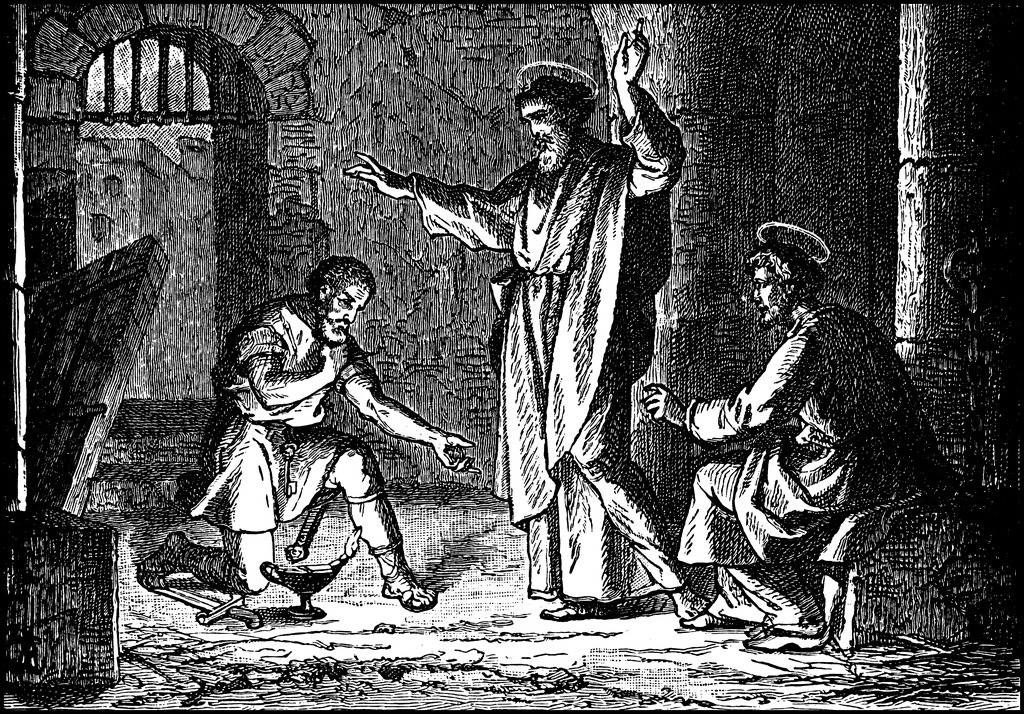
\includegraphics[width=\textwidth]{StsPaulAndSilasInPrison}
\end{center}

\hspace{0pt}
\vfill

\pagebreak

\vspace*{7.5cm}
``Sts. Paul and Silas, being in prison praying, praised God at midnight, and then the earth quaked, and all the prison doors opened, and all fetters and bonds of prisoners were loosed. Our Lord Jesus Christ also prayed, not only in one part of the night, but all the night He woke in prayer, as the Gospel tells... furthermore, some say that for at the time of \textit{Matins}, there appeared a star in the firmament whereby shipmen are ruled in the sea, and bring themselves to right haven; and for our merciful Lady is that star which succours mankind in the troublesome sea of this world, and bringeth her lovers to the haven of health, therefore it is worthy that she be served and praised at the time of \textit{Matins}.'' (Paraphrased from the \textit{Mirror of Our Lady}.) O most Blessed Virgin, with you as the star we set our coruse on life's tempestuous seas, may we , like Sts. Paul and Silas, follow Our Lord's example and keep vigil in prayer, ever wakeful for His coming. Amen.
\vfill

\pagebreak

\chapter*{Before Matins}

\section*{Preparatory Prayers}

\textit{All kneel and pray silently. As you say the prayer \textnormal{Aperi, Domine}, make the sign of the cross with your thumb first over your lips, and then over your heart.}

\begin{latinenglishequalsection}

\latinenglishequal{
	Áperi, {\color{red}\maltese}\ Dómine, os meum ad benedicéndum\linebreak nomen sanctum tuum:
	{\color{red}\maltese}\ munda quoque cor meum ab ómnibus vanis, pervérsis et aliénis cogitatiónibus;
	intelléctum illúmina, afféctum inflámma, ut digne, atténte ac devóte hoc Offícium beátæ Vírginis Maríæ recitáre váleam,
	et exaudíri mérear ante conspéctum divínæ Majestátis tuæ.
	Per Christum Dóminum nostrum. 
	Amen.
}{
	Open, {\color{red}\maltese}\ O Lord, my mouth to bless Thy holy Name; {\color{red}\maltese}\ cleanse also my heart from all vain, evil, and wandering thoughts; enlighten my understanding and kindle my affections; that I may worthily, attentively, and devoutly say this Office of the Blessed Virgin Mary, and so merit to be heard before the presence of Thy divine Majesty.  Through Christ our Lord.  Amen.
}

\latinenglishequal{
	Domine, in unióne illíus divínæ intentiónis, qua ipse in terris laudes Deo persolvísti, has tibi Horas persólvo.
}{
	O Lord, in union with that divine intention wherewith thou, whilst here on earth, didst render praises unto God, I desire to offer this my Office of prayer unto thee.
}

\latinenglishequal{
	Ave María, grátia plena, Dóminus tecum. Benedíc\-ta tu in muliéribus, et benedíctus fructus ventris tui, Jesus.
 Sancta María, Mater Dei, ora pro nobis peccatóribus, nunc et in hora mortis nostræ. Amen.
 }{
 	Hail Mary, full of grace, the Lord is with thee. Blessed art thou among women, and blessed is the fruit of thy womb, Jesus.
 Holy Mary, Mother of God, pray for us sinners, now and at the hour of our death. Amen.
 }
 
 \end{latinenglishequalsection}
 
\chapter*{Matins}

\begin{latinenglishsection}

\heading{\section*{Invitatory}}

\rubric{\color{red}All make the Sign of the Cross as the Officiant says the ``Domine Labia Mea'' and the ``Deus in Adjutorium''. All continue together with the entire ``Gloria Patri'' after the response: }

\latinenglish{
	\gresetinitiallines{1}
	\gregorioscore{domine_labia_mea_aperies}
}{
	{\color{red}\Vbar.} Thou shalt open my lips, {\color{red}\maltese}\ O Lord.\\
	{\color{red}\Rbar.} And my mouth shall shew forth thy prase.
}

\latinenglish{
	\gresetinitiallines{1}
	\gregorioscore{deus_in_adjutorium}
}{
	{\color{red}\Vbar.} O God, {\color{red}\maltese}\ come to my assistance.\\
	{\color{red}\Rbar.} O Lord, make haste to help me.
	
	Glory be to the Father, and to the Son: and to the Holy Spirit; as it was in the beginning, is now, and ever shall be: world without end. Amen. Alleluia.
}

\rubric{\color{red}From Septuagesima until Easter, \textnormal{Alleluia} is replaced with:}

\latinenglish{
	\gresetinitiallines{0}
	\gabcsnippet{
	(c3)Lau(h)s ti(h)bi(h) Dó(h)mi(h)ne(h), Re(h)x æ(h)té(h)rnæ(i) gló(h)ri(h)æ.(g) (::)
	}
}{
	Praise to thee, O Lord, King of everlasting glory.
}

\end{latinenglishsection}

\vfill\pagebreak

%%%%%%%%%%%%%%%%%%%%%%%%%%%%%%%%%%%%%%%%%%%%%%%%%%%%%%%%%%%%%%%%%%%%%

%\section*{THROUGHOUT THE YEAR and CHRISTMASTIDE}

\begin{latinenglishsection}

\rubric{\color{red}The following incipit of the Hail Mary is said \underline{twice}, by the Officiant and Cantor together:}

\latinenglish{
	\gresetinitiallines{1}
	\gregorioscore{ave_maria_gratia_plena}
}{
	Hail Mary, full of grace, the Lord is with thee.
}

\end{latinenglishsection}

\begin{latinenglishsection}

\heading{\section*{Psalm 94}}

\rubric{\color{red}The psalm is said standing. All genuflect at ``Venite adoremus'':}

\latinenglish{
	\gresetinitiallines{1}
	\gregorioscore{venite_exsultemus}
	
}{
	1. O come, let us sing unto The Lord, let us rejoice before God Our Savior:
	let us come into his presence with thanksgiving, and with psalms rejoice before him.
	
	2. {\color{red} Hail Mary, full of grace:
	the Lord is with thee.}
	
	3. For The Lord is a great God, and a great King above all gods: 
	
	4. The Lord will not cast off his people; 
	in his hands are all the ends of the earth, and he beholdeth the heights of the mountains.
	
	5. {\color{red} The Lord is with thee.}
	
	6. The sea is his, and he made it, and his hands founded the dry land:
	
	7. {\color{red}\textit{(genuflect)}}  COME, LET US ADORE AND FALL DOWN BEFORE GOD; 
	{\color{red}\textit{(stand)}} let us lament before the Lord who made us;
	
	8. For he is the Lord Our God:
	we are his people, and the sheep of his pasture.
	
	9. {\color{red} Hail Mary, full of grace:
	 the Lord is with thee.}
	 
	10. Today if ye shall hear his voice:
	harden not your hearts,
	 
	11. As in the provocation, and as in the day of temptation in the wilderness;
	where your fathers tempted me, proved me, and saw my works.
	
	12. {\color{red} The Lord is with thee.}
	
	13. Forty years long was I nigh unto this generation and said:
	They do always err in their heart
	
	14. For they have not known my ways:
	unto whom I sware in my wrath, that they should not enter into my rest.
	
	15. {\color{red} Hail Mary, full of grace,
	the Lord is with thee.}
	
	16. {\color{red}\textit{(bow)}} Glory be to the Father, and to the Son:
	and to the Holy Spirit:
	
	17. {\color{red}\textit{(rise)}} As it was in the beginning, is now:
	and ever shall be, world without end. Amen.
	
	18. {\color{red} The Lord is with thee;
	Hail Mary, full of grace, the Lord is with thee.}
}

\rubric{\color{red}Dóminus tecum. Ave María grátia plena, Dóminus tecum.}

\end{latinenglishsection}

\begin{latinenglishsection}

\heading{\section*{Hymn}}

\rubric{\color{red}The Hymn is lead by the Cantor:}

\latinenglish{
	\gresetinitiallines{1}
	\gregorioscore{quem_terra}
}{
	1. The Lord, whom earth, and sea and sky,
	with one adoring voice proclaim;
	Who rules them all in majesty'
	Enclose'd himself in Mary's frame.
	
	2. Lo! in a humble Virgin's womb,
	O'ershadowed by Almighty power;
	He whom the stars, and sun, and moon,
	Each serve in their appointed hour.
	
	3. O Mother blest! to whom was given
	Within thy body to contain
	The Architect of earth and heaven,
	Whose hand the universe sustain.
	
	4. To thee was sent an angel down;
	In thee the Spirit was enshrine'd;
	Of thee was born that mighty one,
	The long-desir'd of all mankind.
	
	5. O Jesu! born of Virgin bright,
	Immortal glory be to thee;
	Praise to the Father infinite,
	And Holy Ghost eternally. Amen.
}

\rubric{\color{red}Then are said three Psalms, according to the day of the week:}
\rubric{\color{red} Sunday, Monday, and Thursday: \underline{First Nocturn}: next page}
\rubric{\color{red} Tuesday and Friday: \underline{Second Nocturn}: pg. 13}
\rubric{\color{red} Wednesday and Saturday: \underline{Third Nocturn}: pg. 17}

\end{latinenglishsection}

\vfill\pagebreak

\begin{latinenglishsection}

\heading{\section*{First Nocturn}}
\rubric{\color{red}To be said on Sunday, Monday, and Thursday}

\rubric{\color{red}Then Cantor says the antiphon and intones the Psalm up to the asterisk (*), after which all sit. The Cantor, along with his side, finishes the remainder of the first verse, after which either side of the choir alternates between verses. All stand and bow for the ``Gloria Patri''. The remaining Psalms are said in the same manner.}

\heading{\subsection*{Psalm 8}}

\latinenglish{
	\gresetinitiallines{1}
	\gregorioscore{benedicta_tu_intonation}
}{
	Blessed art thou...
}

\latinenglish{
	\gresetinitiallines{1}
	\gregorioscore{psalm_8_1_4ASTAR}
	
	\begin{verses}{1}
	
	\item Quóniam eleváta est magnificén\textit{ti}\textit{a} \textbf{tu}a,~* \textit{su}\textit{per} \textbf{cæ}los.

	\item Ex ore infántium et lacténtium perfecísti laudem propter ini\textit{mí}\textit{cos} \textbf{tu}os,~* ut déstruas inimí\textit{cum} \textit{et} \textit{ul}\textbf{tó}rem.
	
	\item Quóniam vidébo cælos tuos, ópera digitó\textit{rum} \textit{tu}\textbf{ó}rum:~* lunam et stellas, \textit{quæ} \textit{tu} \textit{fun}\textbf{dás}ti.
	
	\item Quid est homo quod me\textit{mor} \textit{es} \textbf{e}jus?~* aut fílius hóminis, quóniam \textit{ví}\textit{si}\textit{tas} \textbf{e}um?
	
	\item Minuísti eum paulo minus ab Angelis,~{\color{red}\GreDagger}\ glória et honóre coro\textit{nás}\textit{ti} \textbf{e}um:~* et constituísti eum super ópera má\textit{nu}\textit{um} \textit{tu}\textbf{á}rum.
	
	\item Omnia subjecísti sub pé\textit{di}\textit{bus} \textbf{e}jus,~* oves et boves univérsas: ínsuper et \textit{pé}\textit{co}\textit{ra} \textbf{cam}pi.
	
	\item Vólucres cæli, et \textit{pi}\textit{sces} \textbf{ma}ris,~* qui perámbulant \textit{sé}\textit{mi}\textit{tas} \textbf{ma}ris.
	
	\item Dómine, Dó\textit{mi}\textit{nus} \textbf{nos}ter,~* {\color{red}\textit{(stand)}} quam admirábile est nomen tuum in u\textit{ni}\textit{vér}\textit{sa} \textbf{ter}ra!
	
	\item {\color{red}\textit{(bow)}} Glória Pa\textit{tri}, \textit{et} \textbf{Fí}lio,~* et Spi\textit{rí}\textit{tu}\textit{i} \textbf{Sanc}to.
	
	\item {\color{red}\textit{(rise)}} Sicut erat in princípio, et \textit{nunc}, \textit{et} \textbf{sem}per,~* et in s\'{\ae}cula sæ\textit{cu}\textit{ló}\textit{rum}. \textbf{A}men.
	
	\end{verses}
	
	\gresetinitiallines{0}
	\gregorioscore{benedicta_tu}
}{
	1. O Lord our Lord, how admirable is thy name in the whole earth! 
	For thy magnificence is elevated above the heavens.

	2. Out of the mouth of infants and of sucklings thou hast perfected praise, because of thy enemies:
	that thou mayst destroy the enemy and the avenger.
	
	3. For I will behold thy heavens, the works of thy fingers: 
	the moon and the stars which thou hast founded.
	
	4. What is man that thou art mindful of him? 
	or the son of man that thou visitest him?
	
	5. Thou hast made him a little less than the angels, thou hast crowned him with glory and honour:
	And hast set him over the works of thy hands.
	
	6. Thou hast subjected all things under his feet:
	all sheep and oxen: moreover the beasts also of the fields.
	
	7. The birds of the air, and the fishes of the sea: 
	that pass through the paths of the sea.
	
	8. O Lord our Lord:
	how admirable is thy name in all the earth!
	
	Glory be to the Father, and to the Son,
	and to the Holy Spirit
	
	As it was in the beginning, is now
	and ever shall be, world without end. Amen.
	
	Blessed art thou among women, and blessed is the fruit of thy womb.
}

\heading{\subsection*{Psalm 18}}

\latinenglish{
	\gresetinitiallines{1}
	\gregorioscore{sicut_myrrha_intonation}
}{
	Like the choicest myrrh...
}

\latinenglish{
	\gresetinitiallines{1}
	\gregorioscore{psalm_18_1_4A}
	
	\begin{verses}{1}
	
	\item Dies diéi e\textit{rúc}\textit{tat} \textbf{ver}bum,~* et nox nocti ín\textit{di}\textit{cat} \textit{sci}\textbf{én}tiam.

	\item Non sunt loquélæ, ne\textit{que} \textit{ser}\textbf{mó}nes,~* quorum non audiántur \textit{vo}\textit{ces} \textit{e}\textbf{ó}rum.
	
	\item In omnem terram exívit so\textit{nus} \textit{e}\textbf{ó}rum:~* et in fines orbis terræ \textit{ver}\textit{ba} \textit{e}\textbf{ó}rum.
	
	\item In sole pósuit taberná\textit{cu}\textit{lum} \textbf{su}um:~* et ipse tamquam sponsus procédens de \textit{thá}\textit{la}\textit{mo} \textbf{su}o.
	
	\item Exsultávit ut gigas ad cur\textit{rén}\textit{dam} \textbf{vi}am,~* a summo cælo e\textit{grés}\textit{si}\textit{o} \textbf{e}jus.
	
	\item Et occúrsus ejus usque ad \textit{sum}\textit{mum} \textbf{e}jus:~* nec est qui se abscóndat a \textit{ca}\textit{ló}\textit{re} \textbf{e}jus.
	
	\item Lex Dómini immaculáta, con\textit{vér}\textit{tens} \textbf{á}nimas:~* testimónium Dómini fidéle, sapiénti\textit{am} \textit{præ}\textit{stans} \textbf{pár}vulis.
	
	\item Justítiæ Dómini rectæ, lætifi\textit{cán}\textit{tes} \textbf{cor}da:~* præcéptum Dómini lúcidum il\textit{lú}\textit{mi}\textit{nans} \textbf{ó}culos.
	
	\item Timor Dómini sanctus, pérmanens in s\'{\ae}\textit{cu}\textit{lum} \textbf{s\'{\ae}}culi:~* judícia Dómini vera, justificáta \textit{in} \textit{se}\textit{met}\textbf{íp}sa.
	
	\item Desiderabília super aurum et lápidem preti\textit{ó}\textit{sum} \textbf{mul}tum:~* et dulcióra su\textit{per} \textit{mel} \textit{et} \textbf{fa}vum.
	
	\item Etenim servus tuus cus\textit{tó}\textit{dit} \textbf{e}a,~* in custodiéndis illis retri\textit{bú}\textit{ti}\textit{o} \textbf{mul}ta.
	
	\item Delícta quis intélligit?~{\color{red}\GreDagger}\ ab occúltis \textit{me}\textit{is} \textbf{mun}da me:~* et ab aliénis par\textit{ce} \textit{ser}\textit{vo} \textbf{tu}o.
	
	\item Si mei non fúerint domináti, tunc immacu\textit{lá}\textit{tus} \textbf{e}ro:~* et emundábor a \textit{de}\textit{líc}\textit{to} \textbf{má}ximo.
	
	\item Et erunt ut compláceant elóquia \textit{o}\textit{ris} \textbf{me}i:~* et meditátio cordis mei in conspéc\textit{tu} \textit{tu}\textit{o} \textbf{sem}per.
	
	\item Dómine, ad\textit{jú}\textit{tor} \textbf{me}us,~* {\color{red}\textit{(stand)}} et \textit{red}\textit{émp}\textit{tor} \textbf{me}us.
	
	\item {\color{red}\textit{(bow)}} Glória Pa\textit{tri}, \textit{et} \textbf{Fí}lio,~* et Spi\textit{rí}\textit{tu}\textit{i} \textbf{Sanc}to.
	
	\item {\color{red}\textit{(rise)}} Sicut erat in princípio, et \textit{nunc}, \textit{et} \textbf{sem}per,~* et in s\'{\ae}cula sæ\textit{cu}\textit{ló}\textit{rum}. \textbf{A}men.
	
	\end{verses}
	
	\gresetinitiallines{0}
	\gregorioscore{sicut_myrrha}
}{
	1. The heavens shew forth the glory of God:
	and the firmament declareth the work of his hands.

	2. Day to day uttereth speech:
	and night to night sheweth knowledge.
	
	3. There are no speeches nor languages:
	where their voices are not heard.
	
	4. Their sound hath gone forth into all the earth:
	and their words unto the ends of the world.
	
	5. He hath set his tabernacle in the sun: 
	and he, as a bridegroom coming out of his bride chamber, 
	
	6. He Hath rejoiced as a giant to run the way:
	His going out is from the end of heaven, 
	
	7. And his circuit even to the end thereof: 
	and there is no one that can hide himself from his heat.
	
	8. The law of the Lord is unspotted, converting souls: 
	the testimony of the Lord is faithful, giving wisdom to little ones.
	
	9. The justices of the Lord are right, rejoicing hearts: 
	the commandment of the Lord is lightsome, enlightening the eyes.
	
	10. The fear of the Lord is holy, enduring for ever and ever: 
	the judgments of the Lord are true, justified in themselves.
	
	11. More to be desired than gold and many precious stones: 
	and sweeter than honey and the honeycomb.
	
	12. For thy servant keepeth them, 
	and in keeping them there is a great reward.
	
	13. Who can understand sins?  from my secret ones cleanse me, O Lord:  
	And from those of others spare thy servant. 
	
	14. If they shall have no dominion over me, then shall I be without spot: 
	and I shall be cleansed from the greatest sin.
	
	15 And the words of my mouth shall be such as may please: 
	and the meditation of my heart always in thy sight. 
	
	16. O Lord, my helper:
	and my redeemer.
	
	Glory be to the Father, and to the Son,
	and to the Holy Spirit
	
	As it was in the beginning, is now
	and ever shall be, world without end. Amen.
	
	Like the choicest myrrh, thou hast yielded an odour of sweetness, O holy Mother of God.
}

\end{latinenglishsection}

\begin{latinenglishsection}

\heading{\subsection*{Psalm 23}}

\latinenglish{
	\gresetinitiallines{1}
	\gregorioscore{ante_torum_intonation}
}{
	Before the couch...
}

\latinenglish{
	\gresetinitiallines{1}
	\gregorioscore{psalm_23_1_4A}
	
	\begin{verses}{1}
	
	\item Quia ipse super mária fun\textit{dá}\textit{vit} \textbf{e}um:~* et super flúmina præ\textit{pa}\textit{rá}\textit{vit} \textbf{e}um.

	\item Quis ascéndet in \textit{mon}\textit{tem} \textbf{Dó}mini?~* aut quis stabit in lo\textit{co} \textit{sanc}\textit{to} \textbf{e}jus?
	
	\item Innocens mánibus et mundo corde,~{\color{red}\GreDagger} qui non accépit in vano á\textit{ni}\textit{mam} \textbf{su}am,~* nec jurávit in dolo \textit{pró}\textit{xi}\textit{mo} \textbf{su}o.
	
	\item Hic accípiet benedictió\textit{nem} \textit{a} \textbf{Dó}mino:~* et misericórdiam a Deo, sa\textit{lu}\textit{tá}\textit{ri} \textbf{su}o.
	
	\item Hæc est generátio quærén\textit{ti}\textit{um} \textbf{e}um,~* quæréntium fáci\textit{em} \textit{De}\textit{i} \textbf{Ja}cob.
	
	\item Attóllite portas, príncipes, vestras,~{\color{red}\GreDagger}\ et elevámini, portæ \textit{æ}\textit{ter}\textbf{ná}les:~* et intro\textit{í}\textit{bit} \textit{Rex} \textbf{gló}riæ.
	
	\item Quis est iste Rex glóriæ?~{\color{red}\GreDagger}\ Dóminus for\textit{tis} \textit{et} \textbf{pot}ens:~* Dóminus \textit{pot}\textit{ens} \textit{in} \textbf{pr\'{\ae}}lio.
	
	\item Attóllite portas, príncipes, vestras,~{\color{red}\GreDagger}\ et elevámini, portæ \textit{æ}\textit{ter}\textbf{ná}les:~* et intro\textit{í}\textit{bit} \textit{Rex} \textbf{gló}riæ.
	
	\item Quis est is\textit{te} \textit{Rex} \textbf{gló}riæ?~* {\color{red}\textit{(stand)}} Dóminus virtútum ip\textit{se} \textit{est} \textit{Rex} \textbf{gló}riæ.
	
	\item {\color{red}\textit{(bow)}} Glória Pa\textit{tri}, \textit{et} \textbf{Fí}lio,~* et Spi\textit{rí}\textit{tu}\textit{i} \textbf{Sanc}to.
	
	\item {\color{red}\textit{(rise)}} Sicut erat in princípio, et \textit{nunc}, \textit{et} \textbf{sem}per,~* et in s\'{\ae}cula sæ\textit{cu}\textit{ló}\textit{rum}. \textbf{A}men.
	
	\end{verses}
	
	\gresetinitiallines{0}
	\gregorioscore{ante_torum}
}{
	1. The earth is the Lord's and the fulness thereof: 
	the world, and all they that dwell therein.

	2. For he hath founded it upon the seas; 
	and hath prepared it upon the rivers.
	
	3. Who shall ascend into the mountain of the Lord: 
	or who shall stand in his holy place?
	
	4. The innocent in hands, and clean of heart:
	who hath not taken his soul in vain, nor sworn deceitfully to his neighbour.
	
	5. He shall receive a blessing from the Lord: 
	and mercy from God his Saviour.
	
	6. This is the generation of them that seek him:
	of them that seek the face of the God of Jacob.
	
	7. Lift up your gates, O ye princes, and be ye lifted up, O eternal gates: 
	and the King of Glory shall enter in.
	
	8. Who is this King of Glory? 
	the Lord who is strong and mighty: the Lord mighty in battle.
	
	9. Lift up your gates, O ye princes, and be ye lifted up, O eternal gates: 
	and the King of Glory shall enter in.
	
	10. Who is this King of Glory? 
	the Lord of hosts, he is the King of Glory.
	
	Glory be to the Father, and to the Son,
	and to the Holy Spirit
	
	As it was in the beginning, is now
	and ever shall be, world without end. Amen.
	
	Before the couch of this Virgin sing often unto us sweet chants with solemnity.
}

\rubric{\color{red}Continue to pg. 21 for the Versicle, the Absolution, and the Lessons.}

\end{latinenglishsection}

\vfill\pagebreak

\begin{latinenglishsection}

\heading{\section*{Second Nocturn}}
\rubric{\color{red}To be said on Tuesday and Friday}

\rubric{\color{red}Then Cantor says the antiphon and intones the Psalm up to the asterisk (*), after which all sit. The Cantor, along with his side, finishes the remainder of the first verse, after which either side of the choir alternates between verses. All stand and bow for the ``Gloria Patri''. The remaining Psalms are said in the same manner.}

\heading{\subsection*{Psalm 44}}

\latinenglish{
	\gresetinitiallines{1}
	\gregorioscore{specie_tua_intonation}
}{
	In thy comeliness...
}

\latinenglish{
	\gresetinitiallines{1}
	\gregorioscore{psalm_44_1_7c}
	
	\begin{verses}{1}
	
	\item Lingua mea \textbf{cá}lamus \textbf{scri}bæ:~* velóci\textbf{ter} scri\textbf{bén}tis.

	\item Speciósus forma præ fíliis hóminum,~{\color{red}\GreDagger}\ diffúsa est grátia in \textbf{lá}biis \textbf{tu}is:~* proptérea benedíxit te Deus \textbf{in} æ\textbf{tér}num.
	
	\item Accíngere gládio tuo super \textbf{fe}mur \textbf{tu}um,~* \textbf{pot}en\textbf{tís}sime.
	
	\item Spécie tua et pulchri\textbf{tú}dine \textbf{tu}a:~* inténde, próspere pro\textbf{cé}de, et \textbf{re}gna.
	
	\item Propter veritátem, et mansuetúdinem, \textbf{et} jus\textbf{tí}tiam:~* et dedúcet te mirabíliter \textbf{déx}tera \textbf{tu}a.
	
	\item Sagíttæ tuæ acútæ, pópuli \textbf{sub} te \textbf{ca}dent:~* in corda inimi\textbf{có}rum \textbf{Re}gis.
	
	\item Sedes tua, Deus, in \textbf{s\'{\ae}}culum \textbf{s\'{\ae}}culi:~* virga directiónis virga \textbf{re}gni \textbf{tu}i.
	
	\item Dilexísti justítiam, et odísti in\textbf{i}qui\textbf{tá}tem:~* proptérea unxit te, Deus, Deus tuus, óleo lætítiæ præ con\textbf{sór}tibus \textbf{tu}is.
	
	\item Myrrha, et gutta, et cásia a vestiméntis tuis, a dómi\textbf{bus} e\textbf{búr}neis:~* ex quibus delectavérunt te fíliæ regum in ho\textbf{nó}re \textbf{tu}o.
	
	\item Astitit regína a dextris tuis in vestítu \textbf{de}au\textbf{rá}to:~* circúmdata va\textbf{ri}e\textbf{tá}te.
	
	\item Audi, fília, et vide, et inclína \textbf{au}rem \textbf{tu}am:~* et oblivíscere pópulum tuum, et domum \textbf{pa}tris \textbf{tu}i.
	
	\item Et concupíscet Rex de\textbf{có}rem \textbf{tu}um:~* quóniam ipse est Dóminus Deus tuus, et ado\textbf{rá}bunt \textbf{e}um.
	
	\item Et fíliæ Tyri \textbf{in} mu\textbf{né}ribus~* vultum tuum deprecabúntur: omnes \textbf{dí}vites \textbf{ple}bis.
	
	\item Omnis glória ejus fíliæ \textbf{Re}gis ab \textbf{in}tus,~* in fímbriis áureis circumamícta va\textbf{ri}e\textbf{tá}tibus.
	
	\item Adducéntur Regi vírgi\textbf{nes} post \textbf{e}am:~* próximæ ejus affe\textbf{rén}tur \textbf{ti}bi.
	
	\item Afferéntur in lætítia et exsul\textbf{ta}ti\textbf{ó}ne:~* adducéntur in \textbf{tem}plum \textbf{Re}gis.
	
	\item Pro pátribus tuis nati sunt \textbf{ti}bi \textbf{fí}lii:~* constítues eos príncipes super \textbf{om}nem \textbf{ter}ram.
	
	\item Mémores erunt \textbf{nó}minis \textbf{tu}i:~* in omni generatióne et gene\textbf{ra}ti\textbf{ó}nem.
	
	\item Proptérea pópuli confitebúntur tibi \textbf{in} æ\textbf{tér}num:~* {\color{red}\textit{(stand)}} et in \textbf{s\'{\ae}}culum \textbf{s\'{\ae}}culi.
	
	\item {\color{red}\textit{(bow)}} Glória \textbf{Pa}tri, et \textbf{Fí}lio,~* et Spi\textbf{rí}tui \textbf{Sanc}to.
	
	\item {\color{red}\textit{(rise)}} Sicut erat in princípio, et \textbf{nunc}, et \textbf{sem}per,~* et in s\'{\ae}cula sæcu\textbf{ló}rum. \textbf{A}men.
	
	\end{verses}
	
	\gresetinitiallines{0}
	\gregorioscore{specie_tua}
}{
	1. My heart hath uttered a good word:
	 I speak my works to the king; 
	 
	 2. My tongue is the pen of a scrivener:
	 that writeth swiftly.

	3. Thou art beautiful above the sons of men: 
	grace is poured abroad in thy lips; therefore hath God blessed thee for ever.

	4. Gird thy sword upon thy thigh, 
	O thou most mighty.

	5. With thy comeliness and thy beauty set out, 
	proceed prosperously, and reign. 
	
	6. Because of truth and meekness and justice: 
	and thy right hand shall conduct thee wonderfully.

	7. Thy arrows are sharp: under thee shall people fall, 
	into the hearts of the king's enemies.

	8. Thy throne, O God, is for ever and ever: 
	the sceptre of thy kingdom is a sceptre of uprightness.

	9. Thou hast loved justice, and hated iniquity: 
	therefore God, thy God, hath anointed thee with the oil of gladness above thy fellows.

	10. Myrrh and stacte and cassia perfume thy garments, from the ivory houses: 
	out of which the daughters of kings have delighted thee in thy glory. 
	
	11. The queen stood on thy right hand, in gilded clothing; 
	surrounded with variety.

	12. Hearken, O daughter, and see, and incline thy ear: 
	and forget thy people and thy father's house.

	13. And the king shall greatly desire thy beauty; 
	for he is the Lord thy God, and him they shall adore.

	14. And the daughters of Tyre with gifts: 
	yea, all the rich among the people, shall entreat thy countenance.

	15. All the glory of the king's daughter is within:
	 in golden borders, clothed round about with varieties. 
	 
	 16. After her shall virgins be brought to the king: 
	 her neighbours shall be brought to thee.

	17. They shall be brought with gladness and rejoicing: 
	they shall be brought into the temple of the king.

	18. Instead of thy fathers, sons are born to thee: 
	thou shalt make them princes over all the earth.

	19. They shall remember thy name throughout all generations. 
	Therefore shall people praise thee for ever; yea, for ever and ever.
	
	Glory be to the Father, and to the Son,
	and to the Holy Spirit.
	
	As it was in the beginning, is now, 
	and ever shall be, world without end. Amen.
	
	In thy comeliness and thy beauty go forth, proceed prosperously and reign.
}

\end{latinenglishsection}

\vfill\pagebreak

\begin{latinenglishsection}

\heading{\subsection*{Psalm 45}}

\latinenglish{
	\gresetinitiallines{1}
	\gregorioscore{adjuvabit_eam_intonation}
}{
	God shall help her...
}

\latinenglish{
	\gresetinitiallines{1}
	\gregorioscore{psalm_45_1_7c}
	
	\begin{verses}{1}
	
	\item Proptérea non timébimus dum tur\textbf{bá}bitur \textbf{ter}ra:~* et transferéntur montes \textbf{in} cor \textbf{ma}ris.

	\item Sonuérunt, et turbátæ sunt \textbf{a}quæ e\textbf{ó}rum:~* conturbáti sunt montes in forti\textbf{tú}dine \textbf{e}jus.
	
	\item Flúminis ímpetus lætíficat civi\textbf{tá}tem \textbf{De}i:~* sanctificávit tabernáculum \textbf{su}um Al\textbf{tís}simus.
	
	\item Deus in médio ejus, non \textbf{com}mo\textbf{vé}bitur:~* adjuvábit eam Deus \textbf{ma}ne di\textbf{lú}culo.
	
	\item Conturbátæ sunt Gentes, et incli\textbf{ná}ta sunt \textbf{re}gna:~* dedit vocem suam, \textbf{mo}ta est \textbf{ter}ra.
	
	\item Dóminus vir\textbf{tú}tum no\textbf{bís}cum:~* suscéptor noster \textbf{De}us \textbf{Ja}cob.
	
	\item Veníte, et vidéte ópera Dómini,~{\color{red}\GreDagger}\ quæ pósuit prodígia \textbf{su}per \textbf{ter}ram:~* áuferens bella usque ad \textbf{fi}nem \textbf{ter}ræ.
	
	\item Arcum cónteret, et con\textbf{frín}get \textbf{ar}ma:~* et scuta com\textbf{bú}ret \textbf{i}gni.
	
	\item Vacáte, et vidéte quóniam \textbf{e}go sum \textbf{De}us:~* exaltábor in Géntibus, et exal\textbf{tá}bor in \textbf{ter}ra.
	
	\item Dóminus vir\textbf{tú}tum no\textbf{bís}cum:~* {\color{red}\textit{(stand)}} suscéptor noster \textbf{De}us \textbf{Ja}cob.
	
	\item {\color{red}\textit{(bow)}} Glória \textbf{Pa}tri, et \textbf{Fí}lio,~* et Spi\textbf{rí}tui \textbf{Sanc}to.
	
	\item {\color{red}\textit{(rise)}} Sicut erat in princípio, et \textbf{nunc}, et \textbf{sem}per,~* et in s\'{\ae}cula sæcu\textbf{ló}rum. \textbf{A}men.
	
	\end{verses}
	
	\gresetinitiallines{0}
	\gregorioscore{adjuvabit_eam}
}{
	1. Our God is our refuge and strength: 
	a helper in troubles, which have found us exceedingly.

	2. Therefore we will not fear, when the earth shall be troubled; 
	and the mountains shall be removed into the heart of the sea.

	3. Their waters roared and were troubled: 
	the mountains were troubled with his strength.

	4. The stream of the river maketh the city of God joyful: 
	the most High hath sanctified his own tabernacle.

	5. God is in the midst thereof, it shall not be moved: 
	God will help it in the morning early.

	6. Nations were troubled, and kingdoms were bowed down: 
	he uttered his voice, the earth trembled.

	7. The Lord of armies is with us: 
	the God of Jacob is our protector.

	8. Come and behold ye the works of the Lord: 
	what wonders he hath done upon earth, making wars to cease even to the end of the earth. 
	
	9. He shall destroy the bow, and break the weapons: 
	and the shield he shall burn in the fire.

	10. Be still and see that I am God; 
	I will be exalted among the nations, and I will be exalted in the earth.

	11. The Lord of armies is with us: 
	the God of Jacob is our protector.

	Glory be to the Father, and to the Son,
	and to the Holy Spirit.
	
	As it was in the beginning, is now, 
	and ever shall be, world without end. Amen.
	
	God shall help her with his countenance: God is in the midst of her, she shall not be moved.
}

%\end{latinenglishsection}

%\vfill\pagebreak

%\begin{latinenglishsection}

\heading{\subsection*{Psalm 86}}

\latinenglish{
	\gresetinitiallines{1}
	\gregorioscore{sicut_laetantium_intonation}
}{
	Our dwelling...
}

\latinenglish{
	\gresetinitiallines{1}
	\gregorioscore{psalm_86_1_7c}
	
	\begin{verses}{1}
	
	\item Gloriósa \textbf{dic}ta sunt \textbf{de} te,~* \textbf{cí}vitas \textbf{De}i.

	\item Memor ero Rahab, et \textbf{Ba}by\textbf{ló}nis~* sci\textbf{én}ti\textbf{um} me.
	
	\item Ecce alienígenæ, et Tyrus, et pópu\textbf{lus} Æ\textbf{thí}opum,~* hi fu\textbf{é}runt \textbf{il}lic.
	
	\item Numquid Sion dicet:~{\color{red}\GreDagger}\ Homo, et homo natus \textbf{est} in \textbf{e}a:~* et ipse fundávit \textbf{e}am Al\textbf{tís}simus?
	
	\item Dóminus narrábit in scriptúris popu\textbf{ló}rum, et \textbf{prín}cipum:~* horum, qui fu\textbf{é}runt in \textbf{e}a.
	
	\item Sicut læ\textbf{tán}tium \textbf{óm}nium:~* {\color{red}\textit{(stand)}} habitáti\textbf{o} est \textbf{in} te.
	
	\item {\color{red}\textit{(bow)}} Glória \textbf{Pa}tri, et \textbf{Fí}lio,~* et Spi\textbf{rí}tui \textbf{Sanc}to.
	
	\item {\color{red}\textit{(rise)}} Sicut erat in princípio, et \textbf{nunc}, et \textbf{sem}per,~* et in s\'{\ae}cula sæcu\textbf{ló}rum. \textbf{A}men.
	
	\end{verses}
	
	\gresetinitiallines{0}
	\gregorioscore{sicut_laetantium}
}{
	1. The foundations thereof are in the holy mountains: 
	The Lord loveth the gates of Sion above all the tabernacles of Jacob.

	2. Glorious things are said of thee, 
	O city of God.

	3. I will be mindful of Rahab:
	and of Babylon knowing me. 
	
	4. Behold the foreigners, and Tyre:
	and the people of the Ethiopians, these were there.

	5. Shall not Sion say: 
	This man and that man is born in her? and the Highest himself hath founded her.

	6. The Lord shall tell in his writings of peoples and of princes, 
	of them that have been in her.

	7. The dwelling in thee:
	is as it were of all rejoicing.

	Glory be to the Father, and to the Son,
	and to the Holy Spirit.
	
	As it was in the beginning, is now, 
	and ever shall be, world without end. Amen.
	
	Our dwelling in thee is as of all those that rejoice, O holy mother of God.	
}

\rubric{\color{red}Continue to pg. 21 for the Versicle, the Absolution, and the Lessons.}

\end{latinenglishsection}

\vfill\pagebreak

\begin{latinenglishsection}

\heading{\section*{Third Nocturn}}
\rubric{\color{red}To be said on Wednesday and Saturday}

\heading{\subsection*{Psalm 95}}

\latinenglish{
	\gresetinitiallines{1}
	\gregorioscore{gaude_maria_intonation}
}{
	Rejoice, O Virgin Mary...
}

\latinenglish{
	\gresetinitiallines{1}
	\gregorioscore{psalm_95_1_4c}
	
	\begin{verses}{1}
	
	\item Cantáte Dómino, et benedícite nó\textit{mi}\textit{ni} \textbf{e}jus:~* annuntiáte de die in diem salutáre \textbf{e}jus.

	\item Annuntiáte inter gentes gló\textit{ri}\textit{am} \textbf{e}jus,~* in ómnibus pópulis mirabília \textbf{e}jus.
	
	\item Quóniam magnus Dóminus, et laudá\textit{bi}\textit{lis} \textbf{ni}mis:~* terríbilis est super omnes \textbf{de}os.
	
	\item Quóniam omnes dii Génti\textit{um} \textit{dæ}\textbf{mó}nia:~* Dóminus autem cælos \textbf{fe}cit.
	
	\item Conféssio, et pulchritúdo in con\textit{spéc}\textit{tu} \textbf{e}jus:~* sanctimónia et magnificéntia in sanctificatióne \textbf{e}jus.
	
	\item Afférte Dómino, pátriæ Géntium,~{\color{red}\GreDagger}\ afférte Dómino glóriam \textit{et} \textit{ho}\textbf{nó}rem:~* afférte Dómino glóriam nómini \textbf{e}jus.
	
	\item Tóllite hóstias, et introíte in á\textit{tri}\textit{a} \textbf{e}jus:~* adoráte Dóminum in átrio sancto \textbf{e}jus.
	
	\item Commoveátur a fácie ejus uni\textit{vér}\textit{sa} \textbf{ter}ra:~* dícite in Géntibus quia Dóminus re\textbf{gná}vit.
	
	\item Etenim corréxit orbem terræ qui non \textit{com}\textit{mo}\textbf{vé}bitur:~* judicábit pópulos in æqui\textbf{tá}te.
	
	\item Læténtur cæli, et exsúltet terra:~{\color{red}\GreDagger}\ commoveátur mare et pleni\textit{tú}\textit{do} \textbf{e}jus:~* gaudébunt campi, et ómnia quæ in \textbf{e}is sunt.
	
	\item Tunc exsultábunt ómnia ligna silvárum a fácie Dómini, \textit{qui}\textit{a} \textbf{ve}nit:~* quóniam venit judicáre \textbf{ter}ram.
	
	\item Judicábit orbem terræ in \textit{æ}\textit{qui}\textbf{tá}te,~* {\color{red}\textit{(stand)}} et pópulos in veritáte \textbf{su}a.
	
	\item {\color{red}\textit{(bow)}} Glória Pa\textit{tri}, \textit{et} \textbf{Fí}lio,~* et Spirítui \textbf{Sanc}to.
	
	\item {\color{red}\textit{(rise)}} Sicut erat in princípio, et \textit{nunc}, \textit{et} \textbf{sem}per,~* et in s\'{\ae}cula sæculórum. \textbf{A}men.
	
	\end{verses}
	
	\gresetinitiallines{0}
	\gregorioscore{gaude_maria}
}{
	1. Sing ye to the Lord a new canticle: 
	sing to the Lord, all the earth.

	2. Sing ye to the Lord and bless his name: 
	shew forth his salvation from day to day.

	3. Declare his glory among the Gentiles: 
	his wonders among all people.

	4. For the Lord is great, and exceedingly to be praised: 
	he is to be feared above all gods.

	5. For all the gods of the Gentiles are devils: 
	but the Lord made the heavens.

	6. Praise and beauty are before him: 
	holiness and majesty in his sanctuary.

	7. Bring ye to the Lord, O ye kindreds of the Gentiles, bring ye to the Lord glory and honour: 
	Bring to the Lord glory unto his name. 
	
	8. Bring up sacrifices, and come into his courts: Adore ye the Lord in his holy court. 
	
	9. Let all the earth be moved at his presence:
	Say ye among the Gentiles, the Lord hath reigned. 
	
	10. For he hath corrected the world, which shall not be moved: 
	he will judge the people with justice.

	11. Let the heavens rejoice, and let the earth be glad, let the sea be moved, and the fulness thereof:
	The fields and all things that are in them shall be joyful. 
	
	12. Then shall all the trees of the woods rejoice before the face of the Lord, because he cometh: 
	because he cometh to judge the earth. 
	
	13. He shall judge the world with justice, 
	and the people with his truth.
	
	Glory be to the Father, and to the Son,
	and to the Holy Spirit.
	
	As it was in the beginning, is now, 
	and ever shall be, world without end. Amen.
	
	Rejoice, O Virgin Mary, thou alone hast destroyed all heresies in all the world.	
}

\heading{\subsection*{Psalm 96}}

\latinenglish{
	\gresetinitiallines{1}
	\gregorioscore{dignare_me_intonation}
}{
	Vouchsafe that I...
}

\latinenglish{
	\gresetinitiallines{1}
	\gregorioscore{psalm_96_1_4c}
	
	\begin{verses}{1}
	
	\item Nubes, et calígo in circú\textit{i}\textit{tu} \textbf{e}jus:~* justítia, et judícium corréctio sedis \textbf{e}jus.

	\item Ignis ante ip\textit{sum} \textit{præ}\textbf{cé}det:~* et inflammábit in circúitu inimícos \textbf{e}jus.
	
	\item Illuxérunt fúlgura ejus \textit{or}\textit{bi} \textbf{ter}ræ:~* vidit et commóta est \textbf{ter}ra.
	
	\item Montes, sicut cera fluxérunt a fá\textit{ci}\textit{e} \textbf{Dó}mini:~* a fácie Dómini omnis \textbf{ter}ra.
	
	\item Annuntiavérunt cæli justí\textit{ti}\textit{am} \textbf{e}jus:~* et vidérunt omnes pópuli glóriam \textbf{e}jus.
	
	\item Confundántur omnes, qui adó\textit{rant} \textit{sculp}\textbf{tí}lia:~* et qui gloriántur in simulácris \textbf{su}is.
	
	\item Adoráte eum, omnes An\textit{ge}\textit{li} \textbf{e}jus:~* audívit, et lætáta est \textbf{Si}on.
	
	\item Et exsultavérunt fí\textit{li}\textit{æ} \textbf{Ju}dæ:~* propter judícia tua, \textbf{Dó}mine:
	
	\item Quóniam tu Dóminus Altíssimus super \textit{om}\textit{nem} \textbf{ter}ram:~* nimis exaltátus es super omnes \textbf{de}os.
	
	\item Qui dilígitis Dóminum, o\textit{dí}\textit{te} \textbf{ma}lum:~* custódit Dóminus ánimas sanctórum suórum, de manu peccatóris liberábit \textbf{e}os.
	
	\item Lux or\textit{ta} \textit{est} \textbf{jus}to,~* et rectis corde læ\textbf{tí}tia.
	
	\item Lætámini, jus\textit{ti} \textit{in} \textbf{Dó}mino:~* {\color{red}\textit{(stand)}} et confitémini memóriæ sanctificatiónis \textbf{e}jus.
	
	\item {\color{red}\textit{(bow)}} Glória Pa\textit{tri}, \textit{et} \textbf{Fí}lio,~* et Spirítui \textbf{Sanc}to.
	
	\item {\color{red}\textit{(rise)}} Sicut erat in princípio, et \textit{nunc}, \textit{et} \textbf{sem}per,~* et in s\'{\ae}cula sæculórum. \textbf{A}men.
		
	\end{verses}
	
	\gresetinitiallines{0}
	\gregorioscore{dignare_me}
}{
	1. The Lord hath reigned, let the earth rejoice: 
	let many islands be glad.

	2. Clouds and darkness are round about him: 
	justice and judgment are the establishment of his throne.
	
	3. A fire shall go before him, 
	and shall burn his enemies round about.
	
	4. His lightnings have shone forth to the world: 
	the earth saw and trembled.
	
	5. The mountains melted like wax, at the presence of The Lord: 
	at the presence of The Lord of all the earth.
	
	6. The heavens declared his justice: 
	and all people saw his glory.
	
	7. Let them be all confounded that adore graven things, 
	and that glory in their idols. 
	
	8. Adore him, all you his angels:
	Sion heard, and was glad. 
	
	9. And the daughters of Juda rejoiced, 
	because of thy judgments, O Lord.
	
	10. For thou art the most high Lord over all the earth: 
	thou art exalted exceedingly above all gods.
	
	11. You that love the Lord, hate evil: 
	the Lord preserveth the souls of his saints, he will deliver them out of the hand of the sinner.
	
	12. Light is risen to the just, 
	and joy to the right of heart.
	
	13. Rejoice, ye just, in the Lord: 
	and give praise to the remembrance of his holiness.
	
	Glory be to the Father, and to the Son,
	and to the Holy Spirit.
	
	As it was in the beginning, is now, 
	and ever shall be, world without end. Amen.
	
	Vouchsafe that I may praise thee, O sacred Virgin: give me strength against thine enemies.	
}

\rubric{\color{red} If the season is Advent, the antiphon for Psalm 97 changes; see pg. 21.}

\heading{\subsection*{Psalm 97 (Throughout the Year and in Christmastide)}}

\latinenglish{
	\gresetinitiallines{1}
	\gregorioscore{post_partum_intonation}
}{
	After child-birth...
}

\latinenglish{
	\gresetinitiallines{1}
	\gregorioscore{psalm_97_1_4c}
	
	\begin{verses}{1}
	
	\item Salvávit sibi déx\textit{te}\textit{ra} \textbf{e}jus:~* et bráchium sanctum \textbf{e}jus.

	\item Notum fecit Dóminus salu\textit{tá}\textit{re} \textbf{su}um:~* in conspéctu Géntium revelávit justítiam \textbf{su}am.
	
	\item Recordátus est misericór\textit{di}\textit{æ} \textbf{su}æ,~* et veritátis suæ dómui \textbf{Is}raël.
	
	\item Vidérunt omnes tér\textit{mi}\textit{ni} \textbf{ter}ræ~* salutáre Dei \textbf{nos}tri.
	
	\item Jubiláte Deo, \textit{om}\textit{nis} \textbf{ter}ra:~* cantáte, et exsultáte, et \textbf{psál}lite.
	
	\item Psállite Dómino in cíthara, in cíthara et \textit{vo}\textit{ce} \textbf{psal}mi:~* in tubis ductílibus, et voce tubæ \textbf{cór}neæ.
	
	\item Jubiláte in conspéctu regis Dómini:~{\color{red}\GreDagger}\ moveátur mare, et pleni\textit{tú}\textit{do} \textbf{e}jus:~* orbis terrárum, et qui hábitant in \textbf{e}o.
	
	\item Flúmina plaudent manu,~{\color{red}\GreDagger}\ simul montes exsultábunt a con\textit{spéc}\textit{tu} \textbf{Dó}mini:~* quóniam venit judicáre \textbf{ter}ram.
	
	\item Judicábit orbem terrárum \textit{in} \textit{jus}\textbf{tí}tia,~* {\color{red}\textit{(stand)}} et pópulos in æqui\textbf{tá}te.
	
	\item {\color{red}\textit{(bow)}} Glória Pa\textit{tri}, \textit{et} \textbf{Fí}lio,~* et Spirítui \textbf{Sanc}to.
	
	\item {\color{red}\textit{(rise)}} Sicut erat in princípio, et \textit{nunc}, \textit{et} \textbf{sem}per,~* et in s\'{\ae}cula sæculórum. \textbf{A}men.
		
	\end{verses}
	
	\gresetinitiallines{0}
	\gregorioscore{post_partum}
}{
	1. Sing ye to the Lord anew canticle: 
	because he hath done wonderful things. 
	
	2. His right hand hath wrought for him salvation, 
	and his arm is holy.

	3. The Lord hath made known his salvation: 
	he hath revealed his justice in the sight of the Gentiles.
	
	4. He hath remembered his mercy: 
	his truth toward the house of Israel. 
	
	5. All the ends of the earth have seen:
	the salvation of our God.
	
	6. Sing joyfully to God, all the earth; 
	make melody, rejoice and sing.
	
	7. Sing praise to the Lord on the harp, on the harp, and with the voice of a psalm:
	With long trumpets, and sound of comet. 
	
	8. Make a joyful noise before the Lord our king:
	Let the sea be moved and the fullness thereof; the world and they that dwell therein.
	
	9. The rivers shall clap their hands and the mountains shall rejoice together at the presence of the Lord: 
	because he cometh to judge the earth. 
	
	10. He shall judge the world with justice, 
	and the people with equity.
	
	Glory be to the Father, and to the Son,
	and to the Holy Spirit.
	
	As it was in the beginning, is now, 
	and ever shall be, world without end. Amen.
	
	After childbirth, thou didst remain a pure virgin: intercede for us, O Mother of God.	
}

\heading{\subsection*{Psalm 97 (Advent)}}

\latinenglish{
	\gresetinitiallines{1}
	\gregorioscore{angelus_domini_intonation}
}{
	The angel of The Lord...
}

\latinenglish{
	\gresetinitiallines{1}
	\gregorioscore{psalm_97_1_1f}
	
	\begin{verses}{1}
	
	\item Salvávit sibi \textbf{déx}tera \textbf{e}jus:~* et bráchium \textit{sanc}\textit{tum} \textbf{e}jus.

	\item Notum fecit Dóminus salu\textbf{tá}re \textbf{su}um:~* in conspéctu Géntium revelávit justí\textit{ti}\textit{am} \textbf{su}am.
	
	\item Recordátus est miseri\textbf{cór}diæ \textbf{su}æ,~* et veritátis suæ dó\textit{mu}\textit{i} \textbf{Is}raël.
	
	\item Vidérunt omnes \textbf{tér}mini \textbf{ter}ræ~* salutáre \textit{De}\textit{i} \textbf{nos}tri.
	
	\item Jubiláte Deo, \textbf{om}nis \textbf{ter}ra:~* cantáte, et exsultá\textit{te}, \textit{et} \textbf{psál}lite.
	
	\item Psállite Dómino in cíthara, in cíthara et \textbf{vo}ce \textbf{psal}mi:~* in tubis ductílibus, et voce \textit{tu}\textit{bæ} \textbf{cór}neæ.
	
	\item Jubiláte in conspéctu regis Dómini:~{\color{red}\GreDagger}\ moveátur mare, et pleni\textbf{tú}do \textbf{e}jus:~* orbis terrárum, et qui hábi\textit{tant} \textit{in} \textbf{e}o.
	
	\item Flúmina plaudent manu,~{\color{red}\GreDagger}\ simul montes exsultábunt a con\textbf{spéc}tu \textbf{Dó}mini:~* quóniam venit judi\textit{cá}\textit{re} \textbf{ter}ram.
	
	\item Judicábit orbem terrárum \textbf{in} jus\textbf{tí}tia,~* {\color{red}\textit{(stand)}} et pópulos in \textit{æ}\textit{qui}\textbf{tá}te.
	
	\item {\color{red}\textit{(bow)}} Glória \textbf{Pa}tri, et \textbf{Fí}lio,~* et Spirí\textit{tu}\textit{i} \textbf{Sanc}to.
	
	\item {\color{red}\textit{(rise)}} Sicut erat in princípio, et \textbf{nunc}, et \textbf{sem}per,~* et in s\'{\ae}cula sæcu\textit{ló}\textit{rum}. \textbf{A}men.
		
	\end{verses}
	
	\gresetinitiallines{0}
	\gregorioscore{angelus_domini}
}{
	1. Sing ye to the Lord anew canticle: 
	because he hath done wonderful things. 
	
	2. His right hand hath wrought for him salvation, 
	and his arm is holy.

	3. The Lord hath made known his salvation: 
	he hath revealed his justice in the sight of the Gentiles.
	
	4. He hath remembered his mercy: 
	his truth toward the house of Israel. 
	
	5. All the ends of the earth have seen:
	the salvation of our God.
	
	6. Sing joyfully to God, all the earth; 
	make melody, rejoice and sing.
	
	7. Sing praise to the Lord on the harp, on the harp, and with the voice of a psalm:
	With long trumpets, and sound of comet. 
	
	8. Make a joyful noise before the Lord our king:
	Let the sea be moved and the fullness thereof; the world and they that dwell therein.
	
	9. The rivers shall clap their hands and the mountains shall rejoice together at the presence of the Lord: 
	because he cometh to judge the earth. 
	
	10. He shall judge the world with justice, 
	and the people with equity.
	
	Glory be to the Father, and to the Son,
	and to the Holy Spirit.
	
	As it was in the beginning, is now, 
	and ever shall be, world without end. Amen.
	
	The angel of The Lord declared unto Mary, and she conceived of the Holy Ghost, (alleluia).	
}

\rubric{\color{red}Continue for the Versicle, the Absolution, and the Lessons.}

%\rubric{\color{red} For the versicles, the Absolution, and the Lessons Throughout the Year and in Christmastide, \underline{see pg. []}.}
%\rubric{\color{red} For the versicles, the Absolution, and the Lessons in Advent, \underline{see pg. []}.}

\end{latinenglishsection}

%%%%%%%%%%%%%%%%%%%%%%%%%%%%%%%%%%%%%%%%%%%%%%%%%%%%%%%%%%%%%%%%%%%%%

\begin{latinenglishsection}

\section*{Versicle}

\rubric{\color{red} The Officiant leads the Versicle, which is solemnized for Sundays and feasts (`Solemn' below) and uses the common tone otherwise (`Common' below).}

\textit{Solemn: Sundays and Feasts}

\latinenglish{
	\gresetinitiallines{0}
	\gabcsnippet{(c3) <c><sp>V/</sp>.</c> Dif(h)fu(h)sa(h) est(h) gra(h)ti(h)a(h) in(h) la(h)bi(h)is(h) tu(h)is.(g'_/hvGF'E/fgf.) (::)}
	
	\gresetinitiallines{0}
	\gabcsnippet{(c3) <c><sp>R/</sp>.</c> Prop(h)te(h)re(h)a(h) be(h)ne(h)di(h)xit(h) te(h) De(h)us(h) in(h) æ(h)ter(h)num.(g'_/hvGF'E/fgf.) (::)}
}{
	{\color{red}\Vbar.} Grace is poured forth on thy lips.\\
	{\color{red}\Rbar.} Therefore hath God blessed thee forever.
}

\end{latinenglishsection}

\begin{latinenglishsection}

\textit{Common:}

\latinenglish{
	\gresetinitiallines{0}
	\gabcsnippet{(c3)<c><sp>V/</sp>.</c> Dif(h)fu(h)sa(h) est(h) gra(h)ti(h)a(h) in(h) la(h)bi(h)is(h) tu(h)is(f). (::)}
	
	\gresetinitiallines{0}
	\gabcsnippet{(c3)<c><sp>R/</sp>.</c> Prop(h)te(h)re(h)a(h) be(h)ne(h)di(h)xit(h) te(h) De(h)us(h) in(h) æ(h)ter(h)num(f). (::)}
}{
	{\color{red}\Vbar.} Grace is poured forth on thy lips.\\
	{\color{red}\Rbar.} Therefore hath God blessed thee forever.
}

\latinenglish{
	%{\color{red}\Vbar.} Diffusa est gratia in labiis tuis.\\
	%{\color{red}\Rbar.} Proptera benedixit te Deus in æternum.\\
	{\color{red}\textit{The Pater Noster is now said in secret, until}}\\
	{\color{red}\Vbar.} Et ne nos inducas in tentationem.\\
	{\color{red}\Rbar.} Sed libera nos a malo.
}{
	%{\color{red}\Vbar.} Grace is poured forth on thy lips.\\
	%{\color{red}\Rbar.} Therefore hath God blessed thee forever.\\
	{\color{red}\textit{The Our Father is now said in secret, until}}\\
	{\color{red}\Vbar.} And lead us not into temptation.\\
	{\color{red}\Rbar.} But deliver us from evil.
}

\end{latinenglishsection}

\vfill\pagebreak

\begin{latinenglishsection}

\section*{The Absolution}

\rubric{\color{red} The Officiant leads the Absolution.}

\latinenglish{
	Precibus et meritis beatæ Mariæ semper Virginis, {\color{red}\GreDagger}\ et omni\textit{um}\\ \textit{Sanc}\textbf{to}rum, perducat nos Dominus ad regna cælorum.\\
	{\color{red}\Rbar.} Amen.\\
	
	{\color{red}\textit{If The Officiant is a priest:}}\\
	{\color{red}\Vbar.} Jube, Domine, benedicere.\\
	
	{\color{red}\textit{If The Officiant is a not a priest:}}\\
	{\color{red}\Vbar.} Jube, Domne, benedicere.
}{
	By the prayers and merits of the Blessed Mary ever Virgin, and aof all the Saints, may the Lord bring us to the Kingdom of Heaven.\\
	{\color{red}\Rbar.} Amen.\\
	
	{\color{red}\textit{If The Officiant is a priest:}}\\
	{\color{red}\Vbar.} Pray, Lord, a blessing.\\
	
	{\color{red}\textit{If The Officiant is a not a priest:}}\\
	{\color{red}\Vbar.} Pray, Father, a blessing.
}

\end{latinenglishsection}

\begin{latinenglishsection}

\section*{The Blessing}

\rubric{\color{red} The Officiant recites the Blessing in a low recto tono.}

\latinenglish{
	Nos cum prole pia benedicat Virgo Maria.\\
	{\color{red}\Rbar.} Amen.
}{
	May the Virgin Mary, with her loving Child, bless us. {\color{red}\Rbar.} Amen.
}

\rubric{\color{red} For Advent, proceed to \underline{pg. 28}. Otherwise, proceed to the next page.}

\end{latinenglishsection}

\vfill\pagebreak

\begin{latinenglishsection}

\section*{The Lessons (Throughout the Year and in Christmastide)}

\rubric{\color{red} The Officiant leads the Lessons. The `Gloria Patri' in the responsories is \underline{not} said during Advent and from Septuagesima to Easter, except for on Feasts of the Blessed Virgin, the Feast of St. Thomas the Apostle, and the Feast of St. Isaac Jogues and His Companions.  During the times when the `Gloria Patri' is omitted, the Te Deum is also ommitted.}

\subsection*{First Lesson: Sirach 24:11-13}

\latinenglish{
	In omnibus requiem quæsivi, et in hæreditate Domini morabor. {\color{red}\GreDagger}\ Tunc præcepit, et dixit mihi Cre\textit{ator} \textbf{om}nium, et qui creavit me, requievit in tabernaculo meo, et dixit mihi: In Jacob inhabita, et in Israel hereditare, et in electis meis mitte radices.~* Tu autem, Domine, misere nobis.\\
	{\color{red}\Rbar.} Deo gratias.
}{
	In all these I sought rest, and I shall abide in the inheritance of The Lord. Then The Creator of all things commanded, and said to me; and he that made me rested in my tabernacle, and he said to me: Let thy dwelling be in Jacob, and thy inheritance in Israel, and take root in mine elect. But thou, Lord, have mercy on us.\\
	{\color{red}\Rbar.} Thanks be to God.\\
}

\latinenglish{
	\gresetinitiallines{1}
	\gregorioscore{sancta_et_immaculata}
}{
	{\color{red}\Rbar.} O holy and immaculate virgin, with what praises I shall extol thee, I know not: * For he whom the heavens could not contain, rested in thy bosom. {\color{red}\Vbar.} Blessed art thou among women, and blessed is the fruit of thy womb. {\color{red}\Rbar.} For he whom,... (repeated) 
}

\end{latinenglishsection}

\begin{latinenglishsection}

\subsubsection*{Blessing for the First Lesson}

\rubric{\color{red} The Officiant recites the Blessing in a low recto tono.}

\latinenglish{
	{\color{red}\textit{If The Officiant is a priest:}}\\
	{\color{red}\Vbar.} Jube, Domine, benedicere.\\
	
	{\color{red}\textit{If The Officiant is a not a priest:}}\\
	{\color{red}\Vbar.} Jube, Domne, benedicere.\\

	Nos cum prole pia benedicat Virgo Maria.\\
	{\color{red}\Rbar.} Amen.
}{
	{\color{red}\textit{If The Officiant is a priest:}}\\
	{\color{red}\Vbar.} Pray, Lord, a blessing.\\
	
	{\color{red}\textit{If The Officiant is a not a priest:}}\\
	{\color{red}\Vbar.} Pray, Father, a blessing.\\

	May the Virgin Mary, with her loving Child, bless us.\\
	{\color{red}\Rbar.} Amen.
}

\end{latinenglishsection}

%
%%
%%%
%%%%%
%%%%%%
%%%%%%%  END OF FIRST LESSON (THROUGHOUT THE YEAR AND CHRISTMASTIDE)
%%%%%%
%%%%%
%%%%
%%%
%%
%

\begin{latinenglishsection}

\subsection*{Second Lesson: Sirach 24:15-16}

\latinenglish{
	Et sic in Sion firmata sum, et in civitate sanctificata similiter requievi: {\color{red}\GreDagger}\ et in Jerusalem potestas mea. Et radicavi in populo honorificato, {\color{red}\GreDagger}\ et in parte Dei mei hære\textit{ditas} \textbf{il}lius, et in plenitudine Sanctorum detentio mea.~* Tu autem, Domine, miserere nobis.\\
	{\color{red}\Rbar.} Deo gratias.
}{
	And so I was established in Sion, and in the holy city likewise I rested: and my power was in Jerusalem, And I took root in an honorable people, and in the portion of my God his inheritance, and my abode is in the full assembly of Saints. But thou, Lord, have mercy on us.\\
	{\color{red}\Rbar.} Thanks be to God.\\
}

\latinenglish{
	\gresetinitiallines{1}
	\gregorioscore{beata_es}
}{
	{\color{red}\Rbar.} Blessed art thou, O Virgin Mary, who didst bear The Lord, the Creator of the world: * Thou wast the mother of him who made thee, and remainest a virgin forever. {\color{red}\Vbar.} Hail Mary, full of grace, The Lord is with thee. {\color{red}\Rbar.} Thou wast the mother... (repeated)
}

\end{latinenglishsection}

\begin{latinenglishsection}

\subsubsection*{Blessing for the Second Lesson}

\rubric{\color{red} The Officiant recites the Blessing in a low recto tono.}

\latinenglish{
	{\color{red}\textit{If The Officiant is a priest:}}\\
	{\color{red}\Vbar.} Jube, Domine, benedicere.\\
	
	{\color{red}\textit{If The Officiant is a not a priest:}}\\
	{\color{red}\Vbar.} Jube, Domne, benedicere.\\

	Per Virginum Matrem, concedat nobis Dominus salutem et pacem.\\
	{\color{red}\Rbar.} Amen.
}{
	{\color{red}\textit{If The Officiant is a priest:}}\\
	{\color{red}\Vbar.} Pray, Lord, a blessing.\\
	
	{\color{red}\textit{If The Officiant is a not a priest:}}\\
	{\color{red}\Vbar.} Pray, Father, a blessing.\\
	
	Through the Virgin Mother, may The Lord grant unto us salvation and peace.\\
	{\color{red}\Rbar.} Amen.
}

\end{latinenglishsection}

%
%%
%%%
%%%%%
%%%%%%
%%%%%%%  END OF SECOND LESSON (THROUGHOUT THE YEAR AND CHRISTMASTIDE)
%%%%%%
%%%%%
%%%%
%%%
%%
%

\vfill\pagebreak

\begin{latinenglishsection}

\subsection*{Third Lesson: Sirach 24:17-20}

\latinenglish{
	Quasi cedrus exaltata sum in Libano, et quasi cypressus in Monte Sion. {\color{red}\GreDagger}\ Quasi palma exaltata sum in Cades, et quasi plantatio rosæ in Jericho. Quasi oliva pretiosa in campis, et quasi platanus exaltata sum juxta aquam in plateis. {\color{red}\GreDagger}\ Sicut cinnamomum et balsamum aromatizans o\textit{dorem} \textbf{de}di: quasi myrrha electa dedi suavitatem odoris.~* Tu autem, Domine, miserere nobis.\\
	{\color{red}\Rbar.} Deo gratias.
}{
	I was exalted like a cedar in Libanus, and as a cypress tree on Mount Sion. I was exalted like a palm-tree in Cades, and as a rose-plant in Jericho. As a fair olive-tree in the plains, and as a plane tree by the water in the streets, was I exalted. I gave forth a sweet fragrance like cinnamon and aromatic balm: I yielded a sweetness of odour like the choicest myrrh. But thou, Lord, have mercy on us.\\
	{\color{red}\Rbar.} Thanks be to God.\\
}

\rubric{\color{red} The following responsory is only said when the Te Deum is omitted:}

\latinenglish{
	\gresetinitiallines{1}
	\gregorioscore{felix_namque}
}{
	{\color{red}\Rbar.} Surely thou art happy, O holy Virgin Mary, and most worthy of all praise: {\color{red}\Vbar.} For out of thee arose the Sun of justice, * Christ our God. {\color{red}\Vbar.} Pray for the people, mediate for the clergy, intercede for the devoted female sex. Let all experience thy assistance, whoever celebrate thy holy commemoration. {\color{red}\Rbar.} For out of thee... (repeated)\\
	{\color{red}\Vbar.} Glory be to the Father, and to the Son, and to the Holy Spirit.\\
	{\color{red}\Rbar.} Christ our God.
}

\rubric{\color{red}If the Te Deum is omitted, proceed to the Conclusion on pg. 36, otherwise, the Te Deum may be found on pg. 33.}

\end{latinenglishsection}

%
%%
%%%
%%%%%
%%%%%%
%%%%%%%  END OF THIRD LESSON (THROUGHOUT THE YEAR AND CHRISTMASTIDE)
%%%%%%
%%%%%
%%%%
%%%
%%
%

%%%%%%%%%%%%%%%%%%%%%%%%%%%%%%%%%%%%%%%%%%%%%%%%%%%%%%%%%%%%%5

\begin{latinenglishsection}

\vfill\pagebreak

\section*{The Lessons (Advent)}

\rubric{\color{red} The Officiant leads the Lessons. The `Gloria Patri' in the responsories is \underline{not} said, except for on Feasts of the Blessed Virgin, the Feast of St. Thomas the Apostle, and the Feast of St. Isaac Jogues and His Companions.  There is no Te Deum.}

\subsection*{First Lesson: Luke 1:26-28}

\latinenglish{
	Missus est Angelus Gabriel a Deo in civitatem Galilææ, cui nomen\\ Nazareth, ad Virginem desponsatam viro cui nomen erat Jospeh, et domo David; {\color{red}\GreDagger}\ et nomen Virginis Maria. Et ingressus Angelus ad eam, dixit: Ave, gratia plena, Do\textit{minus} \textbf{te}cum: benedicta tu in mulieribus.~* Tu autem, Domine, misere nobis.\\
	{\color{red}\Rbar.} Deo gratias.
}{
	The Angel Gabriel was sent from God into a city of Galilee, called Nazareth, to a Virgin espoused to a man whose name was Joseph, of the House of David; and the Virgin's name was Mary. And the Angel being come in, said unto her: Hail, full of grace, The Lord is with thee: blessed art thou among women. But thou, Lord, have mercy on us.\\
	{\color{red}\Rbar.} Thanks be to God.\\
}

\latinenglish{
	\gresetinitiallines{1}
	\gregorioscore{missus_est_gabriel}
}{
	{\color{red}\Rbar.} The Angel Gabriel was sent to Mary, a virgin espoused to Joseph, announcing to her the word, and the Virgin was afraid at the light. Fear not, Mary, thou hast found grace with the Lord * Behold, thou shalt conceive, and bear a son, and he shall be called the Son of the Most High. {\color{red}\Vbar.} The Lord God shall give unto him the throne of David his father, and he shall regin in the house of Jacob forever {\color{red}\Rbar.} Behold, thou shalt conceive,... (repeated) 
}

\end{latinenglishsection}

\begin{latinenglishsection}

\subsubsection*{Blessing for the First Lesson}

\rubric{\color{red} The Officiant recites the Blessing in a low recto tono.}

\latinenglish{
	{\color{red}\textit{If The Officiant is a priest:}}\\
	{\color{red}\Vbar.} Jube, Domine, benedicere.\\
	
	{\color{red}\textit{If The Officiant is a not a priest:}}\\
	{\color{red}\Vbar.} Jube, Domne, benedicere.\\

	Ipso Virgo virginum intercedat pro nobis ad Dominum.\\
	{\color{red}\Rbar.} Amen.
}{
	{\color{red}\textit{If The Officiant is a priest:}}\\
	{\color{red}\Vbar.} Pray, Lord, a blessing.\\
	
	{\color{red}\textit{If The Officiant is a not a priest:}}\\
	{\color{red}\Vbar.} Pray, Father, a blessing.\\

	May the Virgin of virgins herself intercede for us with The Lord.\\
	{\color{red}\Rbar.} Amen.
}

\end{latinenglishsection}

%
%%
%%%
%%%%%
%%%%%%
%%%%%%%  END OF FIRST LESSON (ADVENT)
%%%%%%
%%%%%
%%%%
%%%
%%
%

\vfill\pagebreak

\begin{latinenglishsection}

\subsection*{Second Lesson: Luke 1:29-33}

\latinenglish{
	Quæ cum audisset, turbata est in sermone ejus, et cogitabat qualis esset ista salutatio. {\color{red}\GreDagger}\ Et ait Angelus ei: Ne timeas, Maria; invenisti enim gratiam apud Deum: {\color{red}\GreDagger}\ Ecce concipies in utero, et paries filium, et vocabis nomen ejus Jesum. Hic erit magnus, et Filius Altissimi vocabitur. Et dabit illi Dominus Deus sedem David patris ejus et regnabit in domo Jacob \textit{in æ}\textbf{ter}num, et regni ejus non erit finis.~* Tu autem, Domine, miserere nobis.\\
	{\color{red}\Rbar.} Deo gratias.
}{
	And when she had heard these things, she was troubled at his saying, and thought with herself what manner of salutation this should be. And the Angel said unto her: Fear not, Mary, for thou hast found grace with God. Behold, thou shalt conceive in thy womb, and shalt bring forth a son, and thou shalt call his name Jesus. He shall be great, and shall be called the Son of the Most High. And The Lord God shall give unto him the throne of David his father, and he shall reign in the house of Jacob forever and of his kingdom there shall be no end. But thou, Lord, have mercy on us.\\
	{\color{red}\Rbar.} Thanks be to God.\\
}

\latinenglish{
	\gresetinitiallines{1}
	\gregorioscore{ave_maria_spiritus}
}{
	{\color{red}\Rbar.} Hail Mary, full of grace, the Lord is with thee. * The Holy Ghost shall come upon thee, and the power of the Most High shall overshadow thee: for the Holy which shall be born of thee shall be called the Son of God. {\color{red}\Vbar.} How shall this be done, seeing I know not man? And the Angel answering said unto her: {\color{red}\Rbar.} The Holy Ghost shall come upon thee... (repeated)
}

\end{latinenglishsection}

\begin{latinenglishsection}

\subsubsection*{Blessing for the Second Lesson}

\rubric{\color{red} The Officiant recites the Blessing in a low recto tono.}

\latinenglish{
	{\color{red}\textit{If The Officiant is a priest:}}\\
	{\color{red}\Vbar.} Jube, Domine, benedicere.\\
	
	{\color{red}\textit{If The Officiant is a not a priest:}}\\
	{\color{red}\Vbar.} Jube, Domne, benedicere.\\

	Per Virginum Matrem, concedat nobis Dominus salutem et pacem.\\
	{\color{red}\Rbar.} Amen.
}{
	{\color{red}\textit{If The Officiant is a priest:}}\\
	{\color{red}\Vbar.} Pray, Lord, a blessing.\\
	
	{\color{red}\textit{If The Officiant is a not a priest:}}\\
	{\color{red}\Vbar.} Pray, Father, a blessing.\\
	
	Through the Virgin Mother, may The Lord grant unto us salvation and peace.\\
	{\color{red}\Rbar.} Amen.
}

\end{latinenglishsection}

%
%%
%%%
%%%%%
%%%%%%
%%%%%%%  END OF SECOND LESSON (ADVENT)
%%%%%%
%%%%%
%%%%
%%%
%%
%

\vfill\pagebreak

\begin{latinenglishsection}

\subsection*{Third Lesson: Luke 1:34-38}

\latinenglish{
	Dixit autem Maria ad Angelum: Quomodo fiet istud, quoniam virum non cognosco? {\color{red}\GreDagger}\ Et respondens Angelus, dixit et: Spiritus Sanctus superveniet in te, et virtus Altissimi obumbrabit tibi. Ideoque et quod nascetur ex te Sanctum, vocabitur Filius Dei. Et ecce Elizabeth, cognata tua, et ipsa concepit filium in senectute sua, {\color{red}\GreDagger}\ et hic mensis sextus est illi, quæ vocatur sterilis; quia non erit impossibile apud Deum omne verbum. Dixit autem Maria: Ecce an\textit{cilla} \textbf{Do}mini: fiat mihi secundum verbum tuum.~* Tu autem, Domine, miserere nobis.\\
	{\color{red}\Rbar.} Deo gratias.
}{
	And Mary said to the Angel: How shall this be done, seeing I know not man? And the Angel answering said unto her: The Holy Ghost shall come upon thee, and the power of the Most High shall overshadow thee. And therefore also the Holy which shall be born of thee shall be called the Son of God. And behold, thy cousin Elizabeth, she also hath conceived a son in her old age, and this is the sixth month with her, who is called barren; for no word shall be impossible with God. And Mary said: Behold the handmaid of The Lord, be it done to me according to thy word. But thou, Lord, have mercy on us.\\
	{\color{red}\Rbar.} Thanks be to God.\\
}

\rubric{\color{red} Since the Te Deum is omitted, the following responsory takes its place (the `Gloria Patri' is said in this instance):}

\latinenglish{
	\gresetinitiallines{1}
	\gregorioscore{suscipe_verbum}
}{
	{\color{red}\Rbar.} Receive, O Virgin Mary, the word which hath been communicated to thee by The Lord through the Angel: thou shalt conceive, and bear a son, who shall be both God and man: * That thou mayest be called blessed among all women. {\color{red}\Vbar.} Yea, thou shalt bear a son, and shalt suffer no detriment in thy virginity: thou shalt be with child, and shalt become a mother, remaining ever a virgin undefiled. {\color{red}\Rbar.} That thou mayest be called... (repeated)\\
	{\color{red}\Vbar.} Glory be to the Father, and to the Son, and to the Holy Spirit.\\
	{\color{red}\Rbar.} That thou mayest be called...
}

\rubric{\color{red}Proceed to the Conclusion on pg. 36.}

\end{latinenglishsection}

%
%%
%%%
%%%%%
%%%%%%
%%%%%%%  END OF THIRD LESSON (ADVENT)
%%%%%%
%%%%%
%%%%
%%%
%%
%

\begin{latinenglishsection}

\section*{The Te Deum}

\rubric{\color{red} The Te Deum \underline{is not said} in Advent, or from Septuagesima until Easter, except on Feasts of the Blessed Virgin, the Feast of St. Thomas the Apostle, and the Feast of St. Isaac Jogues and His Companions.}

\latinenglish{
	\gresetinitiallines{1}
	\gregorioscore{te_deum}
}{
	O God, we praise Thee:
	and acknowledge Thee to be the supreme Lord. 
	
	Everlasting Father:
	all the earth worships Thee. 
	
	All the Angels:
	the heavens and all angelic powers, 
	
	All the Cherubim and Seraphim:
	continuously cry to Thee: 
	
	Holy, Holy, Holy:
	Lord God of Hosts! 
	
	Heaven and earth are full:
	of the Majesty of Thy glory. 
	
	The glorious choir of the Apostles: 
	praise thee
	
	The wonderful company of Prophets: 
	praise thee
	
	The white-robed army of Martyrs: 
	praise Thee. 
	
	Holy Church throughout the world:
	acknowledges Thee
	
	The Father of infinite Majesty; 
	
	Thy adorable, true and only Son; 
	
	Also the Holy Spirit, the Comforter. 
	
	O Christ, Thou art the King of glory! 
	
	Thou art the everlasting Son of the Father. 
	
	When Thou tookest it upon Thyself to deliver man, 
	Thou didst not disdain the Virgin's womb. 
	
	Having overcome the sting of death:
	Thou opened the Kingdom of Heaven to all 
	believers. 
	
	Thou sitest at the right hand of God:
	in the glory of the Father. 
	
	We believe that Thou willst come:
	to be our Judge. 
	
	We, therefore, beg Thee to help Thy servants:
	whom Thou hast redeemed with Thy Precious Blood. 
	
	Let them be numbered with Thy Saints:
	in everlasting glory.
	
	Save Thy people, O Lord:
	and bless Thy inheritance! 
	
	Govern them: 
	and raise them up forever.
	
	Day by day:
	we magnify thee.
	
	And we praise Thy Name forever: 
	yes, forever and ever.
	
	Vouchsafe, O Lord, this day:
	to keep us without sin.
	
	Have mercy on us, O Lord: 
	have mercy on us.
	
	Let Thy mercy, O Lord, be upon us:
	for we have hoped in Thee. 
	
	O Lord, in Thee I have put my trust; 
	let me never be put to shame.
}

\rubric{\color{red}Proceed to the Conclusion on the next page.}

\end{latinenglishsection}

\vfill\pagebreak

\begin{latinenglishsection}

\section*{Conclusion}

\rubric{\color{red} Ordinarily, Lauds follows immediately. If Lauds is not said afterwards, the following prayers may be used as a conclusion, and lead by the Officiant.}

\latinenglish{
	{\color{red}\Vbar.} Domine exaudi orationem mean.\\
	{\color{red}\Rbar.} Et clamor meus ad te veniat.\\
	
	Oremus.
	Deus, qui de beatæ Mariæ Virginis utero Verbum tuum, angelo nuntiante, {\color{red}\GreDagger}\ crnem suscipere voluisti; præsta supplicibus tuis, ut qui vere eam Genitricem De\textit{i cre}\textbf{di}mus, ejus apud te intercessionibus adjuvemur~* Per eumdem Dominum nostrum Jesum Christum filium tuum, qui tecum vivit et regnat in unitate Spiritu Sancti, Deus, per omnia  s\'{\ae}cula sæcu\textit{ló}rum.\\
	{\color{red}\Rbar.} Amen.
}{
	{\color{red}\Vbar.} O Lord, hear my prayer.\\
	{\color{red}\Rbar.} And let my cry come unto thee.\\
	
	Let us pray.
	O God, who wast pleased that thy Word, at the message of an angel, should take flesh in the womb of the Blessed Virgin Mary; grant to us, thy humble servants, that, as we believe her to be truly the Mother of God, we may be assisted also by her intercessions with thee. Through the same Lord Jesus Christ, thy Son, who liveth and reigneth with thee in the unity of the Holy Spirit, God, world without end.\\
	{\color{red}\Rbar.} Amen.
}

\end{latinenglishsection}

\begin{latinenglishsection}

\subsection*{The Benedicamus}

\rubric{\color{red} The Benedicamus is that of the common tone, except when during Paschal time:}

\latinenglish{
	\gresetinitiallines{0}
	\gabcsnippet{(c3) <c><sp>V/</sp>.</c> Do(g)mi(h)ne(h) e(h)xau(h)di(g) o(g)ra(g)ti(h)ó(h)nem(h) me(hg)am.(g) (::)}

	\gresetinitiallines{0}
	\gabcsnippet{(c3) <c><sp>R/</sp>.</c> Et(g) cla(h)mor(h) me(h)us(g) ad(g) te(g) vé(h)ni(h)at.(h) (::)}
}{
	{\color{red}\Vbar.} O Lord, hear my prayer.
	{\color{red}\Rbar.} And let my cry come unto thee.
}

\latinenglish{
	\gresetinitiallines{0}
	\gabcsnippet{(c3)<c><sp>V/</sp>.</c> Be(h)ne(h)di(h)cá(h)mus(h) Dó(f)mi(ef)no.(f.) (::)}
	
	\gresetinitiallines{0}
	\gabcsnippet{(c3)<c><sp>R/</sp>.</c> De(h)o(h) grá(f)ti(ef)as.(f.) (::)}
}{
	
	{\color{red}\Vbar.} Let us bless the Lord.
	{\color{red}\Rbar.} Thanks be to God.
}

\end{latinenglishsection}

\begin{latinenglishsection}

\rubric{\color{red}In Paschal Time:}

\latinenglish{
	\gresetinitiallines{0}
	\gregorioscore{benedicamus_paschal}
}{
	{\color{red}\Vbar.} Let us bless the Lord.
	{\color{red}\Rbar.} Thanks be to God.
}

\end{latinenglishsection}

\begin{latinenglishsection}

\rubric{\color{red} The Officiant says the following in a low recto tono:}

\latinenglish{
	\gresetinitiallines{0}
	\gabcsnippet{(c3) <c><sp>V/</sp>.</c> Fi(f)dé(f)li(f)um(f) á(f)ni(f)mæ(f) per(f) mi(f)se(f)ri(f)cór(f)di(f)am(f) De(f)i(f), re(f)qui(f)é(f)scant(f) in(f) pa(f)ce(f.). (::) <c><sp>R/</sp>.</c> Am(f.)en.(f.) (::)}
}{
	{\color{red}\Vbar.} May the souls of the faithful departed, through the mercy of God, rest in peace.
	{\color{red}\Rbar.} Amen.
}
	
\end{latinenglishsection}

\end{document}